% ****** Start of file apssamp.tex ******
%
%   This file is part of the APS files in the REVTeX 4.2 distribution.
%   Version 4.2a of REVTeX, December 2014
%
%   Copyright (c) 2014 The American Physical Society.
%
%   See the REVTeX 4 README file for restrictions and more information.
%
% TeX'ing this file requires that you have AMS-LaTeX 2.0 installed
% as well as the rest of the prerequisites for REVTeX 4.2
%
% See the REVTeX 4 README file
% It also requires running BibTeX. The commands are as follows:
%
%  1)  latex apssamp.tex
%  2)  bibtex apssamp
%  3)  latex apssamp.tex
%  4)  latex apssamp.tex
%
\documentclass[%
 % reprint,
10pt,
superscriptaddress,
twocolumn,
%groupedaddress,
%unsortedaddress,
%runinaddress,
%frontmatterverbose,
%preprint,
%preprintnumbers,
%nofootinbib,
%nobibnotes,
%bibnotes,
 amsmath,amssymb,
 aps,prx,
%pra,
%prb,
%rmp,
%prstab,
%prstper,
%floatfix,
]{revtex4-2}

\usepackage{graphicx}% Include figure files
\usepackage{dcolumn}% Align table columns on decimal point
\usepackage{bm}% bold math
\usepackage{xcolor}
\usepackage{hyperref}% add hypertext capabilities
\usepackage{siunitx}% SI units
\usepackage{physics}
\usepackage[utf8]{inputenc}
\usepackage[T1]{fontenc}
\usepackage{lmodern}
\usepackage{amsmath,amsfonts,amssymb}

\newcommand{\ecoli}[0]{\textit{E. coli}} % use \ecoli command to correctly typeset italic E. coli
\newcommand{\degreec}[0]{$^\circ$C}
\newcommand{\ul}[0]{$\mu$l}
\newcommand{\um}[0]{$\mu$m}

\AtBeginDocument{\renewcommand*{\d}{\mathop{\kern0pt\mathrm{d}}\!{}}}
\graphicspath{{figures/}} % set default figure path to figures/, if we store figure files in figures/, we only need to put file name in \includegraphics{filename.pdf}. For supported formats, e.g. pdf and jpg, we can omit the extensions. This enhances the readability of the source.

% Some formatting guidelines
% 1. Start a new line (\n) for each sentence. This is good for synctex (click pdf and find the line in tex), and also good for Git when comparing versions.
% 2. Communicate thoughts in comments. For example, if you think a figure of something is needed but missing some where, put a comment and describe the needs.
% 3. Colored text: I use red text to emphasize that the claim is not fully backed by our results. The wording may be modified in the future.
% 4. Figure crossref: at the beginning of a sentence, use "Figure~\ref{}". Otherwise, use "Fig.~\ref{}". Note that the "~" is to prevent line breaking in the middle of the crossref.

% Some content problems that need to be fixed
% 1. Same quantities are referred to in different notations, e.g. \tau^* and \tilde{\tau}, x and y, \tilde{D} and D_A



\begin{document}

\preprint{APS/123-QED}

\title{Bacterial Dynamics in Curved Spaces}% Force line breaks with \\

\author{Cristian Villalobos Concha}
\author{Maria Luisa Cordero}
\author{Rodrigo Soto}
\affiliation{Departamento de Física, FCFM, Universidad de Chile, Santiago, Chile.}

% \altaffiliation[Also at ]{Laboratoire Gulliver, UMR 7083 CNRS, ESPCI Paris, PSL Research University, 75005 Paris, France.}%Lines break automatically or can be forced with \\
\author{Anke Lindner}
\author{Eric Clément}
\affiliation{%
 Laboratoire PMMH, UMR 7636 CNRS-ESPCI-Sorbonne Université-Université Paris Diderot, 7-9 quai Saint-Bernard, 75005 Paris, France.
 }%

\author{Teresa Lopez-Leon}

\affiliation{Laboratoire Gulliver, UMR 7083 CNRS, ESPCI Paris, PSL Research University, 75005 Paris, France.}
\date{\today}
% It is always \today, today,
%  but any date may be explicitly specified
\author{Zhengyang Liu}

\affiliation{%
 Laboratoire PMMH, UMR 7636 CNRS-ESPCI-Sorbonne Université-Université Paris Diderot, 7-9 quai Saint-Bernard, 75005 Paris, France.
 }%
\affiliation{Laboratoire Gulliver, UMR 7083 CNRS, ESPCI Paris, PSL Research University, 75005 Paris, France.}

\begin{abstract}
The interplay between complex environments and active matter suggests a possibility to control and engineer active matter by carefully designing the confinement structures.
It is now well established that confinement may influence transport, rheology, pressure, spatial distribution and collective motion of active matter.
Curved confining walls, which are ubiquitous in biological systems, show their own, specific rich and intriguing effects on active matter.
Here, using a double emulsion system, where the inner and outer droplet sizes can be independently controlled, we experimentally investigate the influence of curved confinement on an active bath of \textit{Escherichia coli} (\ecoli) bacteria.
In particular, we analyze the fluctuations of the inner droplet using the framework of a stochastic ``active noise'' model, and show that the strength of active noise is not an intrinsic property of an active bath, but depends on the confinement curvature.
\textcolor{red}{Our numerical simulations revealed the origin of this dependence on confinement.}
Our results pose new challenge to active matter theory and suggest new methods to control active matter.

\end{abstract}

%\keywords{Suggested keywords}%Use showkeys class option if keyword
                              %display desired
\maketitle

\section{Introduction}
% Use "Active noise" key word to label all the literatures related to this project
The interactions between active and passive objects are always intriguing.
On the one hand, passive objects are often used as a probe to assess the properties, in particular activity, which are sometimes challenging to measure directly.
On the other hand, the capabilities of activity to ehance mixing of fluids and transport of nutrients show great ecological significance and can potentially enable important biomedical applications \cite{Kurtuldu2011, Pushkin2013, Saintillan2008a, Sokolov2009a}.

On the most elementary level, the interaction between an active particle and a passive particle can be described as ``scattering''.
In this process, the active particle swims by the passive particle results in a closed-loop trajectory, due to the hydrodynamic head-rear symmetry of the model swimmer \cite{Dunkel2010}.
In the presence of a confining wall, the flow field generated by an active swimmer is modified, as if there is a mirror image of the swimmer, with force singularities pointing in opposite directions \cite{Blake1974}.
The head-rear symmetry is broken in the modified flow field, leading to net displacement of passive object in a single scattering event.
Based on this picture, Mino et al. successfully modeled the confinement effect on the diffusivity of passive particles in active bath \cite{Mino2011, Mino2013}.
\citet{Lagarde2020} focused their experiment more on the single scattering event, and found far field hydrodynamic interactions to be irrelevant compared to direct collisions.
The experiments mentioned above all revealed an important aspect of active baths: the effect on passive tracer diffusivity is stochastic and additive.
This discovery has led to efforts to model active baths as a stochastic noise \cite{Gregoire2001, Maggi2014, Wu2000, Ye2020}.

Boundaries are known to have dramatic impact on active matter, with examples of pattern formation, directed flow and unusual mechanical properties \cite{Wioland2013, Wu2017, Liu2019}.
Planar boundaries, which are common and easy to produce in labs, have been studied extensively in the past two decades.
However, less is known about how curved boundaries affect active matter behavior.

In this paper, we experimentally investigate this question by putting active bacterial suspensions into the middle layer (also know as the ``shell'' layer) of oil-water-oil double emulsions.
We analyze the fluctuations of the inner droplet using the framework of a stochastic ``active noise'' model, and show that the strength of active noise is not an intrinsic property of an active bath, but depends on the confinement curvature.
\textcolor{red}{Furthermore, we show that the dependence on confinement originates from two aspects: collision angle and activity. Our numerical simulations reveal the origin how spherical confining wall reduces the activity of an active bath.}
Our results deepen the understanding of active matter behavior under confinement.

\section{Experiment}
% Initial version is copied from Overleaf

\begin{figure*}[!t]
  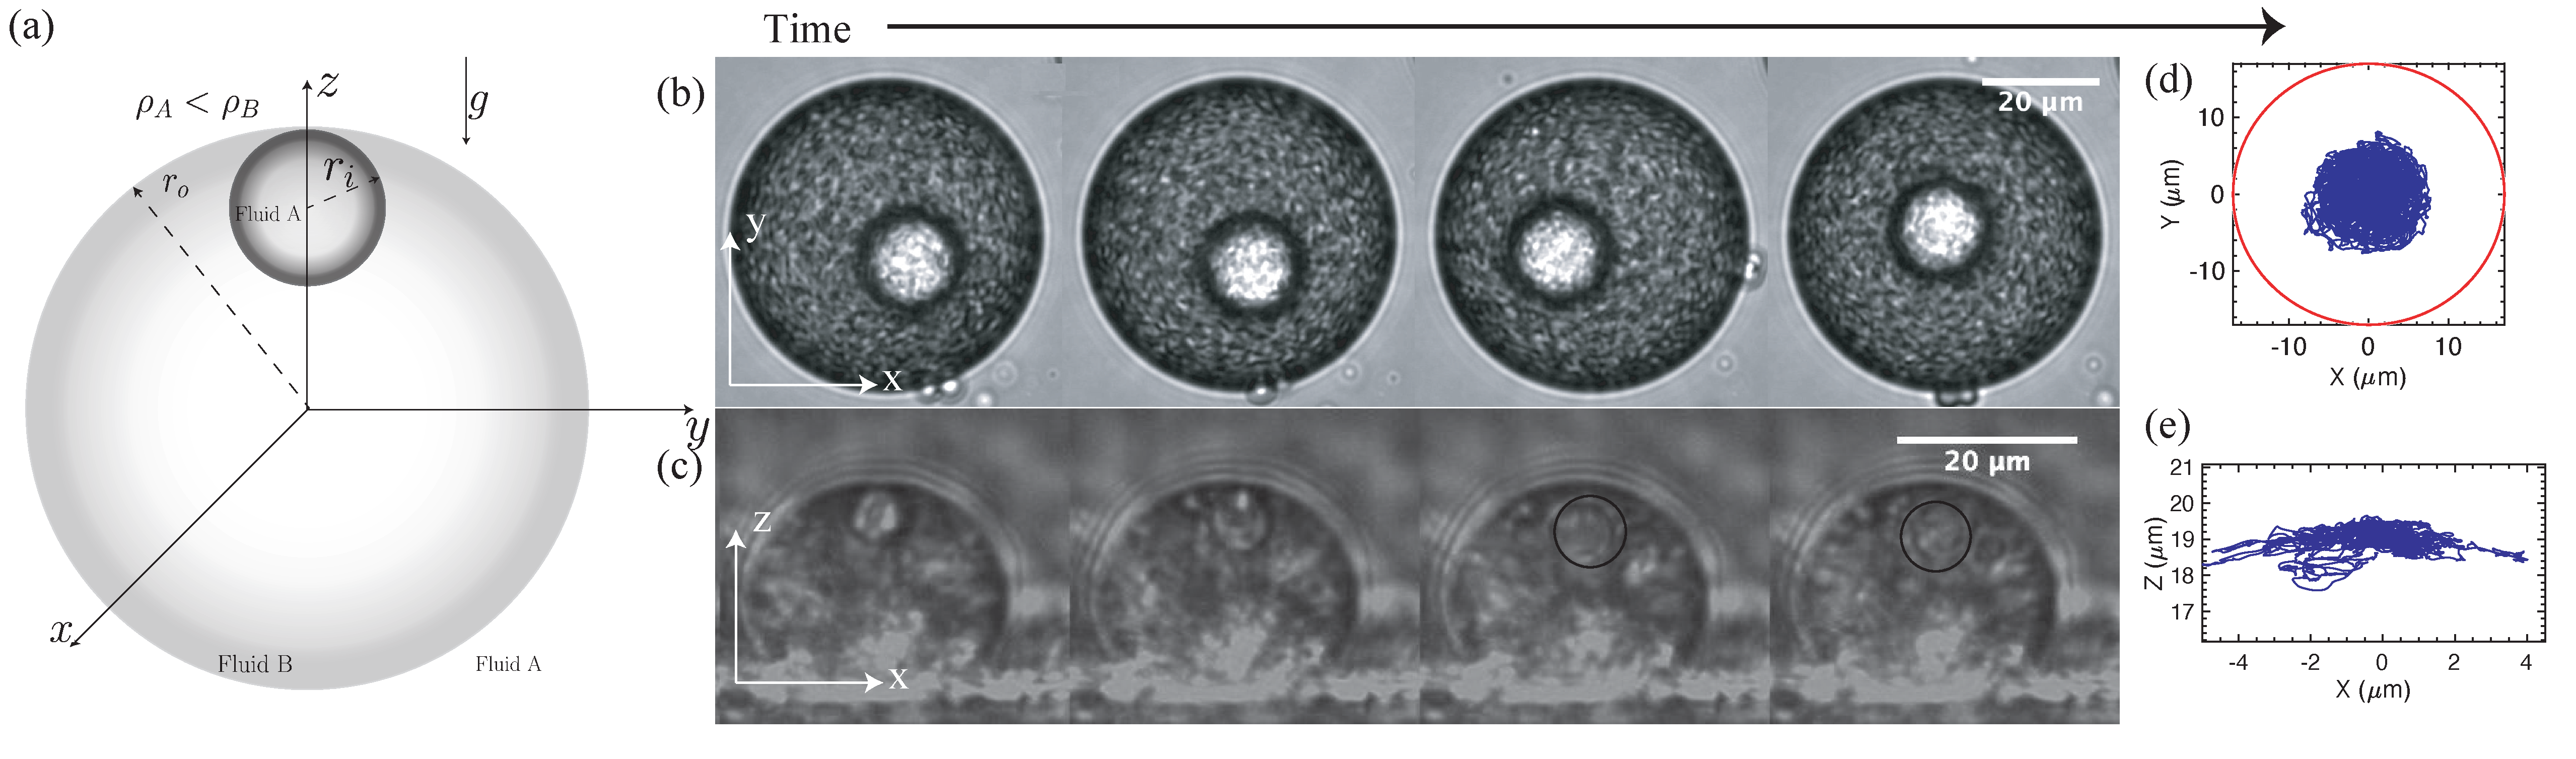
\includegraphics[width=\textwidth]{Diagrama_DE}
  \caption{
  \textbf{Double emulsion --- bacterial shells.}
  (a) A Schematic diagram of the bacterial shell system, along with the coordinate system defined on it.
  The outer droplet of density $\rho_A$ and radius $r_o$ filled with bacterial suspensions.
  Inside this droplet there is another droplet filled with an oil of density $\rho_B < \rho_A$.
  (b) Sequence of image separated by $\Delta t =\SI{5}{\second}$. Top row; shows the XY plane of a bacterial shell of outer diameter $r_o=\SI{27}{\micro\meter}$ and a inner droplet of diameter $r_i=\SI{13.5}{\micro\meter}$.
  (c) A view of the XZ plane of a drop of diameter $r_o=\SI{11.5}{\micro\meter}$ and a inner drop of $r_i=\SI{2.9}{\micro\meter}$.
  (d-e) Trajectory of the center of the inner droplet.
  }
  \label{montaje_doble}
\end{figure*}

\subsection{Bacterial culture}

Wild-type \ecoli bacteria (strain  W3110) were grown with a standard culturing protocol \cite{Keymer2008}.
10 \ul~of frozen stock stored at -20\degreec~was diluted in 10 ml of lysogenic broth (LB) and incubated overnight in a shaking incubator at temperature 30\degreec~and 210 rpm. 
The overnight culture was then diluted in 100 times in LB and let grow for 3.5 hours to reach the optical density at 600 nm (OD) of $0.6\pm 0.1$. 
Bacteria were harvested by centrifuging the suspensions at 2100 $g$ for 10 min. 
Then the supernatant was removed, and the pellet was resuspended in a minimal motility buffer, MMA (10 mM potassium phosphate, 0.1 mM EDTA and 10 mM sodium lactate \cite{Minamino2003}).
\textcolor{red}{In the droplet experiments, I used the MB described in Eric's protocol. The most nominal difference is the addition of L-serine.} 
In MMA, bacteria are allowed to swim, but not to divide. 
The final concentration of the bacterial suspensions ranges from $OD = 0.7$ to $OD = 100$.
\subsection{Double emulsion}

Double emulsions were produced by mechanical mixing of the aqueous bacterial suspension and hexadecane (Sigma-Aldrich, H6703).
10 \ul~bacterial suspension was added to 1 ml hexadecane containing 2 wt\% Span 80 (Sigma-Aldrich, S6760) as a surfractant. 
1 wt\% polyvinyl alcohol (PVA, $M_w$ 13,000-23,000, Sigma-Aldrich, 363170) was supplemented to the oil phase to stabilize the inner droplets.
The mixture is mannually agitated to form many aqueous droplets in oil, among which 10\% are with another oil droplet inside.
Since this is an emulsion inside another emulsion, we term this experimental system a double emulsion, which is illustrated in Fig.~\ref{montaje_doble}(a).
The double emulsion was then diluted 1:10 in hexadecane for observaton.
This dilution ensured enough space between droplets, so that hydrodynamic interactions can be neglected. 

\subsection{Microscopy}

The same photoprinted square observation chamber was used in this work (described in \citet{Ramos2020}).
The chamber was loaded with 200~\ul~of the double emulsion and subsequently sealed with a coverslip to minimize evaporation.
Due to density mismatch between water and hexadecane, the aqueous droplets sedimented to the bottom of the chamber, while the inner oil droplets floated to the top of the aqueous droplets.  
The chamber was then placed on an inverted microscope (Nikon Ti-XX) and the double emulsions were filmed with XX camera at 50-70 Hz.
The $xz$-plane observation was achieved by a microscope sitting on a rotating ``cradle'' (described in XX). 
Magnifications ranging from 20X to 60X were used in our experiments, depending on the size of the droplets. 
Figures~\ref{montaje_doble}(b) and (c) show some snapshots of $xy$-plane and $xz$-plane videos, respectively. 

\subsection{Image analysis}

Droplet tracking was done with a method based on Hough Transform (HT), a common technique for feature extraction \cite{Stockman2001}. 
The results were refined by a custom Python code, which will be discussed in the appendix.
Particle image velocimetry (PIV) was performed using OpenPIV package in Python \cite{OpenPIV}, for characterizing bacterial activity in droplets.


\section{Results}
% I'm not sure if I have to have a dedicated section to discuss the results.
\subsection{Inner droplet trajectories}

In the double emulsion experimental system, the inner droplet is frequently ``kicked'' by the many swimming bacteria around it.
As a result, it exhibits fluctuations much stronger than Brownian motion in the horizontal ($y$) direction.
Due to the smaller density of the inner droplet relative to the bacterial suspension, a buoyant force is constantly pushing it to the top surface of the outer droplet, making the dome an equilibrium position.
In the vertical ($z$) direction, the inner droplet mostly follows the outer droplet surface.
A typical inner droplet trajectory is shown in Fig.~\ref{fig:traj-analysis}(a).
The colored dots denote the positions of inner droplet center at different time.
In cases where inner droplet size is very small, while the bacterial activity is large, inner droplet can leave the surface.
We can roughly estimate the critical inner droplet radius, below which bacterial activity can overcome buoyant force.
The buoyant force is $F_b = \frac{4}{3}\pi r_i^3\Delta\rho g$, where $\Delta\rho\approx 230$ kg/m$^3$ is the density difference between water and hexadecane, and $g\approx 9.8$ m/s$^2$ is the gravitational accelaration.
The propelling force of a single bacteria is approximated by the Stokes drag on a sphere $F_a \approx 6\pi\eta r_b V_b$, where $\eta=0.001$ Pa$\cdot$s is water viscosity, $r_b\approx 0.5$ $\mu$m is bacteria cross section radius and $V_b \approx 20$ $\mu$m/s is the simming speed of bacteria.
Let $F_b=F_a$, we get a critical droplet radius $r_c \approx 2.7$ $\mu$m.
Indeed, since we never prepared inner droplet with radius $r_i < r_c$, inner droplet leaving the surface is a rare event.
However, in very concentrated bacterial suspensions, the inner droplet can leave the surface even when $r_i > r_c$.
This is likely due to more frequent collision events, or collective motions.

\begin{figure*}[!t]
  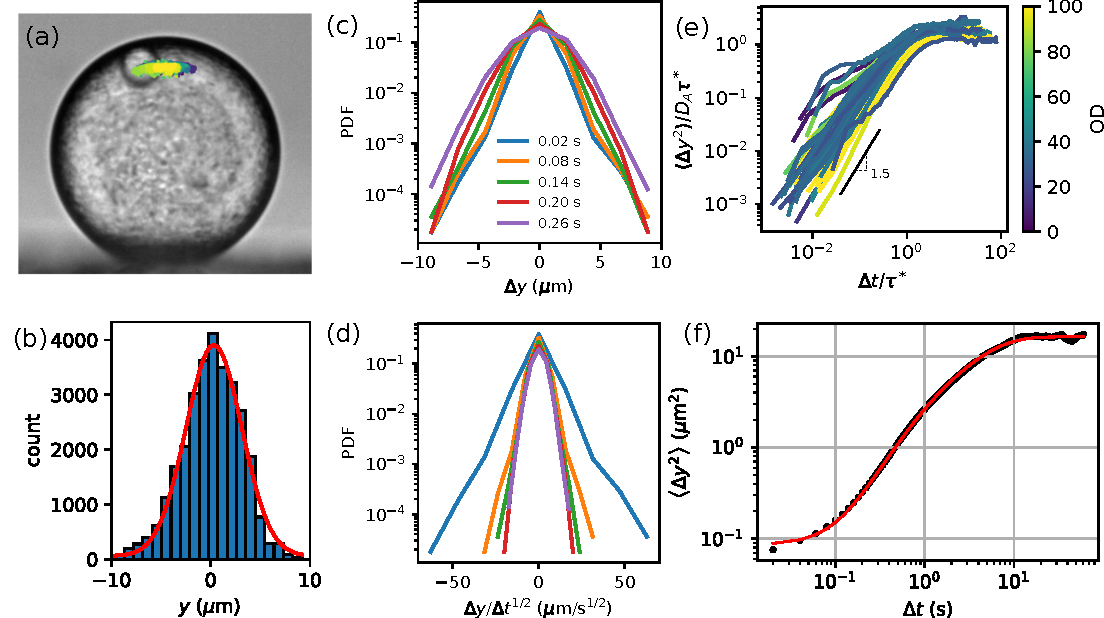
\includegraphics[width=\textwidth]{2-traj-analysis}
  \caption{
  \textbf{Inner droplet trajectory analysis.}
  (a) The trajectory of the inner droplet plotted on an experimental image.
  Outer droplet radius $r_o= 33.2$ $\mu$m and inner droplet radius $r_i=6.0$ $\mu$m.
  Color from dark purple to bright yellow denotes time from the beginning to the end.
  (b) Position probability distribution in $y$ direction. Red curve is a Gaussian fit to the distribution, with mean $\mu = -0.3$ $\mu$m and standard deviation $\sigma = 2.8$ $\mu$m.
  (c) Displacement probability density function (PDF) in $y$ direction, at various time interval $\Delta t$.
  (d) Displacement PDF, where the displacement $\Delta y$ is rescaled by the square root of time interval $\Delta t^{1/2}$.
  (e) Mean square displacement (MSD) of all inner droplet trajectories in this study, with time rescaled by fitted relaxation time $\tau^*$ and MSD rescaled by the product of active diffusivity and relaxation time $D_A\tau^*$.
  (f) A fit of MSD data to our 1D model, fitting parameters are $D_A=1.95$ $\mu$m$^2$/s, $\tau=0.25$ s, $\tau^*=4.40$ s and $c=0.086$ $\mu$m$^2$/s.
  }
  \label{fig:traj-analysis}
\end{figure*}

Next, we measured the position and displacement probability distribution functions (PDF) in the horizontal direction, as shown in Figs.~\ref{fig:traj-analysis}(b-d).
The distribution is well fitted by a Gaussian function, shown as the red curve.
According to \citet{Leptos2009}, in the presence of swimmers, the displacement PDF is characterized by a Gaussian core and exponential tails.
In our data, exponential tails are also observed when $\Delta t = 0.02, 0.08, 0.14$ s, manifesting anomalous transport [Fig.~\ref{fig:traj-analysis}(c)].
Further increasing the time interval makes the exponential tails disappear.
\textcolor{red}{When rescaling the displacement $\Delta y$ with square root of time interval $\Delta t^{1/2}$, as shown in Fig.~\ref{fig:traj-analysis}(d), we notice that all the Gaussian cores of the PDF curves, except the $\Delta t=0.02, 0.08$ s ones, collapse on the same master curve.
The deviations of the small $\Delta t$ curves from the master curve suggest that strong persistence is in play at this time scale $\tau_c\approx 0.1$ s, rather than a random diffusive process.}
Finally, we measured the mean square displacement (MSD) of inner droplets in all our experiments, at various bacterial concentrations and droplet sizes, as shown in Fig.~\ref{fig:traj-analysis}(e).
The lag time and MSD are rescaled by $\tau^*$ and $D_A\tau^*$, respectively, which are obtained from fitting the original MSD data to the 1D model described before.
An example of the fit is shown in Fig.~\ref{fig:traj-analysis}(f).
Typically, the MSD is characterized by a superdiffusive regime at small $\Delta t$, and a transition to saturation at large $\Delta t$.
A diffusive regime can be identified in some cases, but not always.
The critical $\Delta t$'s, $\tau$ and $\tau^*$, vary with droplet sizes and possibility bacterial concentrations, which will be discussed in the following section.

\subsection{Confinement effect}

We studied the motions of inner droplets in over 100 systems of various sizes and bacterial concentration.
Although the simple ``mechanical mixing'' technique does not provide accurate control over droplet sizes, we manage to explore a considerable large parameter space in detail, and to reveal the confinement effect.
The explored parameter space is shown in Fig.~\ref{fig:confinement-effect}(a).
Since we have 3 different parameters varying at the same time, we shall select experiments where two of the parameters are fixed, in order to illustrate the effect from a single parameter.
Here, we choose $\text{OD}\in(20, 40]$ (blue pentagons) and $\text{OD}\in(60, 80]$ (green squares) to illustrate low and high bacterial concentrations, respectively.
To see the effect of outer droplet radius $r_o$, we select data where $r_i\in[5, 9]$ ($\mu$m) and plot active diffusivity $D_A$, persistence time $\tau$ and relaxation time $\tau^*$ as functions of $r_o$, as shown in Fig.~\ref{fig:confinement-effect}(b).
We find that $D_A$ increases monotonically with $r_o$ at both low and high OD.
The increasing rate at high OD, characterized by the slope of $D_A$-$r_o$ curve, is much larger than that at low OD.
$\tau$ and $\tau^*$ show little to no dependence on $r_o$ in our experiments.
Similarly, to see the effect of inner droplet radius $r_i$, we select data where $r_o\in[30, 50]$ ($\mu$m) and plot $D_A$, $\tau$ and $\tau^*$ as functions of $r_i$, as shown in Fig.~\ref{fig:confinement-effect}(c).
We find that neither $D_A$ nor $\tau$ show pronounced dependence on $r_i$, while $\tau^*$ decreases monotonically with $r_i$.
Interestingly, $\tau^*$ at different OD's are quite consistent in magnitude.

% I'm not sure if I should discuss the predictions of the model here, or later in another section.

\begin{figure}[!t]
  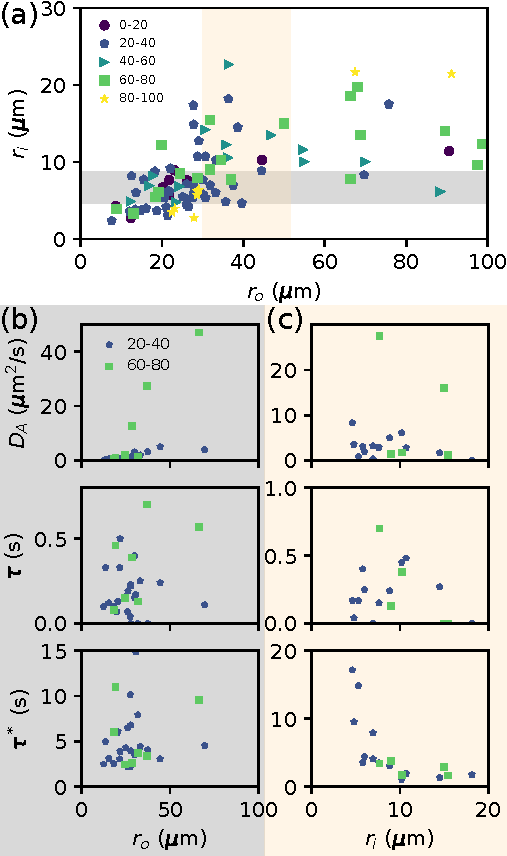
\includegraphics[width=\columnwidth]{3-confinement-effect}
  \caption{
  \textbf{Confinement effect on the inner droplet motions.}
  (a) Explored parameter space of outer droplet radius $r_o$, inner droplet radius $r_i$ and bacterial concentration in terms of optical density (OD).
  OD's are divided in 5 groups, shown as different colors and markers in the plot.
  Two bins of data are selected to highlight the confinement effect.
  The first bin is $r_i\in[5, 9]$ ($\mu$m), as shaded in gray.
  The second bin is $r_o\in[30, 50]$ ($\mu$m), as shaded in light orange.
  (b) Fitting parameters $D_A$, $\tau$ and $\tau^*$ plotted as functions of $r_o$ in the first bin.
  (c) Fitting parameters $D_A$, $\tau$ and $\tau^*$ plotted as functions of $r_i$ in the second bin.
  }
  \label{fig:confinement-effect}
\end{figure}


\subsection{Bacterial activity}

The confinement effect on the active diffusivity may be correlated with the bacterial activity.
Indeed, we frequently observed very different activity at the same bacterial concentration.
In order to quantify the activity, we perform PIV analysis on the bright field images of active double emulsions and use the root mean square of the PIV velocity magnitude as a measure of activity.
Formally, we obtain velocity magnitude field $\mathbb{V}=\{\bm{V}_{i}\}$ from PIV.
The mean velocity $\overline V$ is defined as
%
\begin{equation}
    \overline V = \sqrt{\frac{1}{N}\sum_{i}^N |\bm{V}_{i}|^2}.
\end{equation}
%
To suppress noise from the detection, mean velocities are measured in each pair of frames and then averaged. 
We fix the interrogation window size at 20 pixels throughout all the analyses, with overlap between adjacent windows at 10 pixels.

\begin{figure}[!t]
  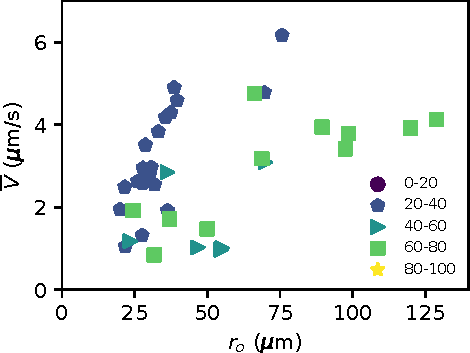
\includegraphics[width=\columnwidth]{bacterial-activity}
  \caption{
  Mean PIV velocity $\overline V$ as a measure of bacterial activity, plotted against outer droplet radius $r_o$.
  }
  \label{fig:bacterial-activity}
\end{figure}

In Fig.~\ref{fig:bacterial-activity}, we plot $\overline V$ as a function of $r_o$.
As usual, the data are put into different groups by bacterial concentrations.
In each OD bin, in particular $\text{OD}\in(20, 40]$ (blue pentagons) and $\text{OD}\in(60, 80]$ (green squares), $\overline V$ increases with $r_o$, suggesting that droplet confinement hinders the activity of bacteria.
However, from this data, it is still unclear how activity depends on OD.

\textcolor{red}{
At the moment, we have not finished PIV on all the videos, partially due to the less organized data analysis in the past.
As a result, we see less data points in Fig.~\ref{fig:bacterial-activity} compared to the parameter space plot Fig.~\ref{fig:confinement-effect}(a).
In addition, I did not have Cristian's raw data from Chile, so it was impossible to apply the same PIV algorithm on both data sets.
Recently, we are transferring the raw videos from Chile to Paris.
In the meantime, I am reorganizing and redoing PIV analysis on the Paris data.
The goal of this reanalysis is to provide better consistency in the method.
For example, when setting interrogation window size, we want the physical size (rather than pixel size) to be constant across all the analysis.
There are also changes in my PIV code, related to smoothing, which can also lead to a difference in the final results.
Last thing is the long standing problem regarding droplet boundary and mask, which also requires uniform treatment.
In short, a REDO of PIV is ongoing, and is likely to change the results given in Fig.~\ref{fig:bacterial-activity}.
When we have the new data, we shall discuss the interpretations and the limitations of the method, and so on.
}
\subsection{Droplet lifetime}
\textcolor{blue}{
In this section, we report the time dependence of droplet activity, in particular the ``frozen droplet'' phenomenon.
We hope to use this phenomenon as a support of our argument that confinement affects bacterial activity.
However, even if this support turns out to be weak, we still can publish this phenomenon on its own, because it's new.
}

It is of key importance to ensure steady state in all active matter experiment.
For bacterial systems, this is particularly challenging, due to the fact that bacteria are very sensitive to their environment, which can change rapidly due to the massive metabolic activities. 
Our experiment typically produce 10-minute videos of active double emulsions. 
A typical bacterial sample used in our experiment, however, can only last around an hour, before the activity decay becomes apparent. 
Therefore, it is necessary to verify the steady state of experiment. 

Water-in-oil emulsion has been used to confine bacteria in many previous experimental works \cite{Hamby2018, Lushi2014, Rajabi2021, Ramos2020, Vincenti2019, Wioland2013}. 
Most of them emphasize that the videos are taken within a very short time after sample preparation, and the activity is in steady state. 
The claimed sample lifetimes are summarized in Table~\ref{tab:sample-lifetime}. Being emphasized many times, steady state and sample lifetime are clearly very crucial to bacterial droplet experiments. 
Yet, further investigation on what determines the sample lifetime is quite rare, especially in droplet. 
There are two reasons: (i) previous experiment does not require very long imaging; (ii) sample lifetime can be affected by many factors, and is therefore difficult to narrow down the scope.

\begin{table}
  \caption{\label{tab:sample-lifetime}Sample lifetime in previous experiments.}
  \begin{ruledtabular}
  \begin{tabular}{lll}
  Bacteria & Video time & Reference \\
  \textit{B. subtilis} & > 10 min & \cite{Wioland2013} \\
  \ecoli & 3 min & \cite{Hamby2018} \\
  \textit{M. gryphiswaldense} & 30 min & \cite{Vincenti2019} \\
  \ecoli & 30 min & \cite{Rajabi2021} \\
  \end{tabular}
  \end{ruledtabular}
\end{table}

In this work, we perform Particle Image Velocimetry (PIV) to quantify the bacterial activity in droplets of various sizes. 
In Fig.~\ref{fig:lifetime}(a), we show how mean velocity evolves over time, up to 50 minutes. 
Generally, the curves starts with a steady state, followed by a rapid decay.
When droplets are small ($r_o<25$ $\mu$m), it is difficult to identify a steady state and we always observe activity decay from the very beginning of experiments.
As a result, the lifetime of bacterial droplets, which is defined as the time it takes for the mean velocity to decay to half of the initial value, depends on droplet size. 
In Fig.~\ref{fig:lifetime}(b), we plot droplet lifetime as a function of droplet size. 
We observe that droplet lifetime generally increases with droplet size, and the time scale is on the order of 10 minutes, in agreement with previous works. 
It is well known that blue light generates unfavorable substances that hinders bacterial motility \cite{bergColiMotion2004}.
Therefore, we also briefly explore the effect of blue light exposure. 
Normally, the samples are subject to continuous light exposure, and the corresponding lifetime data are plotted in black markers in Fig.~\ref{fig:lifetime}(b).
To test the light effect, two samples are only exposed to light intermittently, and the corresponding lifetime data are plotted in red markers in Fig.~\ref{fig:lifetime}(b).
The data suggest that less exposure to blue light leads to a considerable increase of droplet lifetime.
Droplet size and blue light exposure might work in a convoluted way, which is not clear so far.

\begin{figure}[!t]
  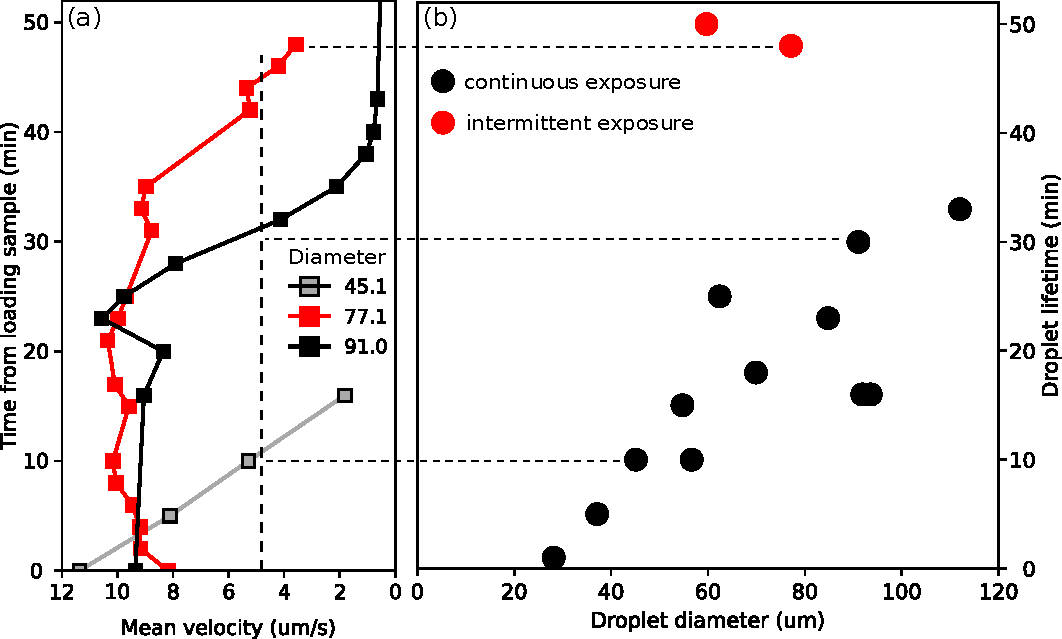
\includegraphics[width=\columnwidth]{droplet-lifetime}
  \caption{
  (a) Mean PIV velocity $\overline V$ as a measure of bacterial activity, plotted against time after loading the samples to sealed observation chambers.
  (b) Droplet lifetime, defined as the time it takes for the mean velocity to decay to half of the initial value, as a function of droplet diameter. 
  The effect of light exposure is briefly explored. 
  Continuous exposure data - the default light condition - are plotted in black markers.
  Intermittent exposure data, where the light is only on for 10/120 seconds, are plotted in red markers.
  }
  \label{fig:lifetime}
\end{figure}

% I want to improve the structure of the paper.
% Currently, we have 
% Introduction
% Experiment
% Results
%   - numerical simulation (duplicate) 
% Simulation results (duplicate)
% Discussions
% Appendix

% The two simulation results look duplicate and I want to merge them
% Tentatively, I remove section simulation results and put all the contents under Results/numerical simulation.

\subsection{Numerical simulation}
% Idea is to align some simulation results with experimental results.
% The current simulation is good on its own, but lacks some alignment with experiment, for example the parameters.
% If there are new results from simulation, we can get together to discuss what to include in this section.
% Here I will write the details of the model, and then summarize that in the main text.
\textit{Methods - }To describe the motion of a particle of density $\rho_i$, radii $r_i$ immersed in a bacterial bath with viscosity $\eta$ and density $\rho_0$ which is confined in a spherical domain of radii $r_o$ and density $\rho_0$.
We propose a Langevin equation with an active noise produced by the bacterial bath and reflective boundary condition. 
This noise is modeled as an colored noise with zero mean.
The boundary condition for the particle can be written as follow: $x^2+y^2+z^2\leq (r_o-r_i)^2$, which mean that in any time $t$ the particle is inside the sphere.  
The equation of motion in the limit of low Reynolds number is 
\begin{align}\label{eq.Langevin_num}
  \mathbf{\dot{r}}=\mathbf{u}(t)-v_s\mathbf{\hat{z}},
\end{align}
where  $v_s=2 r_i^2 \Delta\rho g/9\eta$ is the sedimentation velocity of the particle.
It can be shown that a colored noise is produced by a random motion with white noise, e.g. an Uhlenbeck-Ornstein process:
\begin{align}\label{OUP}
  \dot{u}&=-\frac{u}{\tau}+\frac{\xi(t)}{\tau},
\end{align}
where $\xi(t)$ is a white noise with zero mean and variance delta:
\begin{align}
  \langle \xi(t)\rangle &=0,\\
  \langle \xi(t)\xi(t')\rangle &=2v^2\tau\delta(t-t').
\end{align}
The second moment of the velocity is:
\begin{align}
  \langle u(t)u(t')\rangle &=v_b^2e^{-|t-t'|/\tau},
\end{align}
which is the velocity autocorrelation function of this velocity field.
To solve this system numerically, we used the Euler-Maruyama method for stochastic differential equations.
As we mention before, we can produce an exponentially time correlated noise from a Ornstein-Uhlenbeck process.
Using Euler, we solve for the position of the particle and the noise for the time step $n$.
\begin{align}
   \label{eq:Euler_method}
   x_n&=x_{n-1}+u_{x_{n-1}}\dd t,\\
   y_n&=y_{n-1}+u_{y_{n-1}}\dd t,\\
   z_n&=z_{n-1}+(u_{z_{n-1}}-v_s)\dd t,\\
   u^i_{n}&=u^i_{n-1}-\frac{1}{\tau}u^i_{n-1}dt+\frac{1}{\tau}v\sqrt{2\Delta t}N^i_{n},
\end{align}
where $N^{i}_n$ is a random number with zero mean and variance one.

The simulation has four independent variables $r_o,r_i,v_b^2,\tau$. 
The idea here is to check under which condition the input parameters of the bath $v_b, \tau$, remain the same when we extract this values from the model. Equation \ref*{MSD} explicitly show $v_b^2$ and $\tau$, but this is for the case of a point particle in the presence of the bath. So lets re-writte \textcolor{red}{Eq.XX} to:

\begin{equation}
	\label{MSD_fit}
	=\frac{2v_{\text{fit}}^2}{(\frac{1}{\tilde{\tau}_{\text{fit}}}+\frac{1}{\tau}_{\text{fit}})}\left[\frac{(1-e^{-\frac{2}{\tilde{\tau}_{\text{fit}}} t})}{\frac{2}{\tilde{\tau}_{\text{fit}}}}-\frac{(e^{-(\frac{1}{\tilde{\tau_{\text{fit}}}}+\frac{1}{\tau_{\text{fit}}})t}-e^{-\frac{2t}{\tilde{\tau}_{\text{fit}}} })}{\frac{1}{\tilde{\tau_{\text{fit}}}}-\frac{1}{\tau}_{\text{fit}}}\right].
\end{equation}

To fit the MSD of the particle, I used the following procedure:
\begin{itemize}
\item From the Slope MSD: $\alpha(t) = \frac{d(\log(\langle \Delta x^2 (t)\rangle))}{d\log(t)}$ find the time when the slope is $\alpha = 1.7$. 
\item Fit the MSD up to $t$ when $\alpha = 1.7$ with the MSD for an Active Brownian Particle (ABP). \textcolor{red}{References for this fitting procedure and model?}

$\left<\Delta x^2\right>= v_b^2\left[t-\tau(1-e^{-t/\tau})\right]$
\item Here extract $v_{\text{fit}}$, $\tau_{\text{fit}}$.
\item Then fit the whole MSD with $v_{\text{fit}}$, $\tau_{\text{fit}}$ fixed to determine $\tilde{\tau}_\text{fit}$
\end{itemize}


\textit{Results - }The results are summarized as follows.
\begin{itemize}
  \item As we vary $r_o$ and keep other variables constant at: $r_i = 10$ $\mu$m, $\tau =1$ s, $v_b =1$ $\mu$m/s, \textcolor{red}{complete with a full description of the results! Please refer to the relevant plots.}

\begin{figure}[h!]
  \centering
  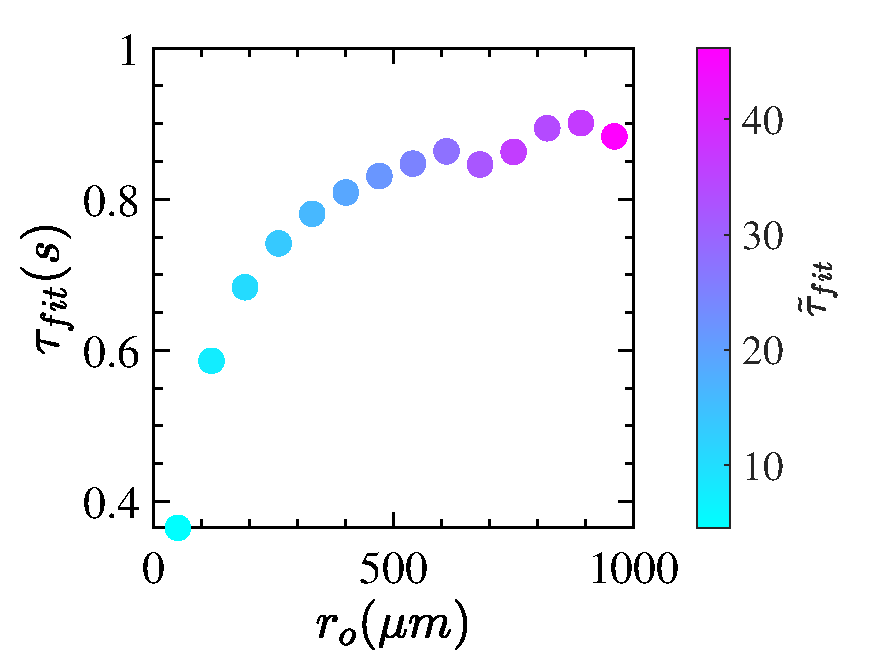
\includegraphics[width=\columnwidth]{ro_t1fit_t2fit}
  \caption{}
  \label{fig:MSD_different_ro}
\end{figure}
\begin{figure}[h!]
  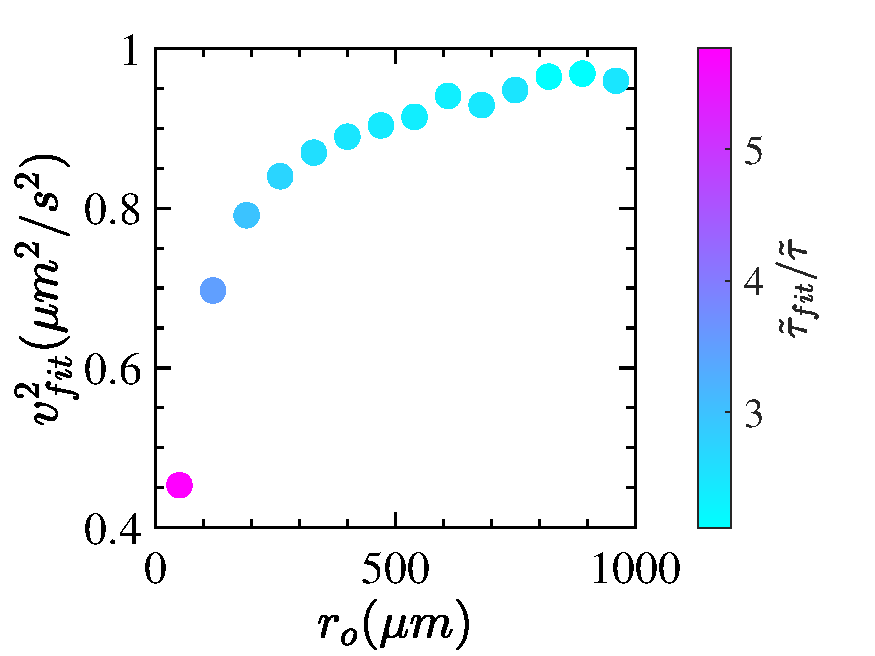
\includegraphics[width=\columnwidth]{ro_v2fit_t2fit}
  \caption{}
  \label{fig:v2_ro}
\end{figure}



\end{itemize}




\section{Discussions}

\textcolor{blue}{
  In this section, we discuss the results. 
  For the results we understand, we can provide more insight, e.g. by giving more detailed description and analysis of a model. 
  For the results we do not understand yet, we discuss in the context of literature, and pose specific open questions for future research to follow up.
}

\subsection{One dimensional model}

The confinement can be approximated to an harmonic potential, which allows us to write a one dimensional equation for the particle moving on the surface of the potential, and this can be solved analytically. \textcolor{red}{I think we need to refer to Maggi's paper and discuss why we use different notations.}

\begin{align}
    \label{eq.Langevin}
    \dot{x}=u(t)-\frac{x}{\tilde{\tau}}.
\end{align}
%
where $\tilde{\tau}=\Gamma/k$, with $\Gamma$ the friction coefficient, $k$ the spring constant for the harmonic potential, and $u(t)$ is the active noise induced by the bacterial suspension.
We will model the active noise as a colored Gaussian noise, with the following statistical properties:
%
\begin{align}
    \label{eq.act.noise}
    \langle u(t)\rangle &=0,\\
    \langle u(t)u(t')\rangle &=v_b^2e^{-|t-t'|/\tau}.
\end{align}
%
where $v_b^2$ is the intensity of the active noise, and $\tau$ is the persistence time of the bacterial fluxes. 
We can solve the equations for the MSD of the particle:
\begin{equation}
	\label{MSD1d}
	\left<\Delta x^2\right>=\frac{2v_b^2}{(\frac{1}{\tilde{\tau}}+\frac{1}{\tau})}\left[\frac{(1-e^{-\frac{2}{\tilde{\tau}} t})}{\frac{2}{\tilde{\tau}}}-\frac{(e^{-(\frac{1}{\tilde{\tau}}+\frac{1}{\tau})t}-e^{-\frac{2}{\tilde{\tau}} t})}{\frac{1}{\tilde{\tau}}-\frac{1}{\tau}}\right].
\end{equation}

The model predicts the geometry dependence of saturation time $\tilde\tau$ explicitly. 
According to Stokes law, $\Gamma = 6\pi\eta r_i$, where $\eta$ is the viscosity of bacterial suspensions. 
The effective spring constant arising from buoyancy and the curved confining wall $k \approx \Delta m g / (r_o - r_i)$, where $\Delta m$ is the buoyant mass of the oil droplet in bacterial suspensions, which can be computed as $\Delta m = \Delta \rho \frac{4}{3}\pi r_i^3$. 
Taken together, $\tilde\tau$ can be expressed as:
$$
\tilde\tau = \frac{9\eta}{2\Delta\rho g}\frac{r_o-r_i}{r_i^2}.
$$
In Fig.~\ref{fig:confinement-effect}, we have shown $\tilde\tau$ as functions of $r_o$ and $r_i$. In the plots, it is observed that $\tilde\tau$ increases with $r_o$ and decreases with $r_i$, agreeing with the predicted trend. To validate the prediction of the model, we can plot $\tilde\tau$ as a function of $(r_o-r_i)/r_i^2$. As shown in Fig.~\ref{fig:sat-time}, the linear-like increasing trend between $\tilde\tau$ and $(r_o-r_i)/r_i^2$ is indeed observed.

\begin{figure}[h!]
  \centering
  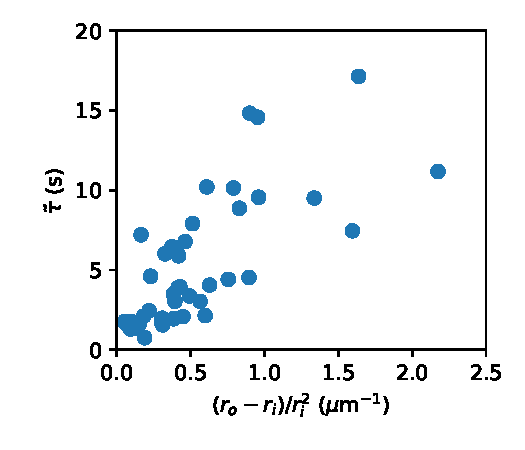
\includegraphics[width=\columnwidth]{saturation-time}
  \caption{Saturation time $\tilde\tau$ as a function of geometrical factor $(r_o-r_i)/r_i^2$.}
  \label{fig:sat-time}
\end{figure}

The data suggests that the prefactor $\frac{9\eta}{2\Delta\rho g}\approx 8$ $\mu$m$\cdot$s.
We can calculate the effective viscosity of bacterial suspensions $\eta\approx 0.004$ Pa$\cdot$s.
This viscosity is slightly larger than water viscosity, suggesting that the presence of swimming bacteria results in more viscous drag on passive objects in the suspension, in intereting contrast with previous findings where pusher type swimmers reduce the viscosity of their suspending fluids \cite{Hatwalne2004, Gachelin2013, Giomi2010, Haines2008, Haines2009, Martinez2020, Slomka2017, Sokolov2009, Lopez2015, Guo2018, Liu2019}. 
\textcolor{red}{Note that for the double emulsion experiments, the motility buffer (MB) is not supplemented with L-serine, so that the viscosity of MB can be well approximated by water viscosity.}
In these works, swimmers need to be aligned by background flows, so that they can collectively generate significant effect on viscosity. 
The absence of such strong alignment may lead to the enhancement of viscosity in our experiment.
A more quantitative account is out of the scope of the present work, but is a worthy question for future investigations.

\subsection{Concentration dependence}

In most active matter experiments and models, the concentration of active particles plays a key role in the behavior of the systems. 
For example, in bacterial suspensions, numerous works have shown that collective motions emerge only if the concentration of bacteria reaches a critical value \cite{Gachelin2014, Peng2021, Liu2021}.
The ability to move passive objects also strongly depends concentration.  
\citet{Mino2011} studied the diffusion of passive particles immersed in \ecoli suspensions near glass surface. 
The results suggested that the enhancement of diffusivity is proportional to the ``active flux'', which is defined as the product of bacterial concentration $n$ and the average swimming speed $v$:
%
\begin{equation}
	\label{eq:active-flux}
	D_A = D_0 + \beta n v ,
\end{equation}
%
where $D_0$ is the thermal diffusivity in the absence of bacteria.
Figure~\ref{fig:collision-angle}(a) shows active diffusivity $D_A$ as a function of bacterial concentration in terms of optical density at 600 nm wavelength, OD.
If we assume the bacterial samples are uniform in terms of activity, similar swimming speed $v$ should be expected, and therefore similar $D_A$ should be expected for same OD. 
However, the data show obvious scattering at all OD's.
For example, when OD$\approx 100$, $D_A$ data span almost 3 orders of magnitude. 
In Fig.~\ref{fig:confinement-effect}(b), we showed that $D_A$ increases with outer droplet size, highlighting a key difference between the present work and \citet{Mino2011}: the outer droplet imposes a curved surface confining the inner droplet and bacteria, which modifies their interactions. 
The most direct consequence is that certain collision angles, which are accessible near flat surface, are no longer accessible in the presence of curved surface.
If a bacterium collides with an inner droplet at an angle $\theta$ with respect to the horizontal plane, as illustrated in Fig.~\ref{fig:collision-angle}(b), only the horizontal component of the swimming speed, $v\cos\theta$, can contribute to moving the droplet. 
To adapt the ``active flux'' model (Eq.~\ref{eq:active-flux}) to our system with a curved surface, we assume that (i) all the bacteria interacting with the inner droplet swim in parallel with the outer droplet surface, and (ii) only the horizontal component of ``flux'' contributes to the inner droplet motion. As a result, Eq.~\ref{eq:active-flux} is modified to
%
\begin{equation}
  \label{eq:active-flux-angle}
  D_A = D_0 + \beta n v \cos\theta = D_0 + \beta n v \frac{\sqrt{(r_o-r_i)^2-r_i^2}}{r_o-r_i}.
\end{equation}
%
Note that when $r>R/2$, the square root above goes imaginary. This corresponds to relatively large inner droplets in our data set. In those cases, the diffusivity $D_A$ is mostly very small (\textcolor{red}{need data support}). Therefore, we use a 2-step function $f(R, r)$ as the correction factor to the model:
%
\begin{equation}
  D_A = D_0 + \beta n v f(R, r),
\end{equation}
%
where
$$
  f(R, r) =
  \begin{cases}
  \frac{\sqrt{(R-r)^2-r^2}}{R-r}, & \text{if}\; r\le R/2 \\
  0, & \text{if}\; r > R/2
  \end{cases}
$$
%

In Fig.~\ref{fig:collision-angle}(c), we plot $D_A$ as a function of OD$\cos\theta$. 
Compared to Fig.~\ref{fig:collision-angle}(a), where collision angle is not considered, the data are brought closer, despite the still significant scattering. 

Up to now, we have been assuming that the swimming speed $v$ is a constant. 
However, our PIV-based bacterial activity measurement in the previous section suggests that swimming speed also depends on the size of out droplet, i.e. $v = v(r_o)$. 
As shown in Fig.~\ref{fig:bacterial-activity}, if we look at a single concentration bracket, it is obvious that the average swimming speed $\overline V$ increases with outer droplet radius $r_o$.
\textcolor{red}{Comparison across different concentration brackets is still problematic. That small OD samples have higher mean velocity compared to large OD samples is counterintuitive and requires reviewing of the data.}
In an attempt to consider this factor, we plot $D_A$ as a function of $\text{OD}\cos\theta r_o^\alpha$ in Fig.~\ref{fig:collision-angle}(d), where $\alpha=0,1,2$.
When $\alpha=1$, the $D_A$ data become less scattered, especially the high OD data, colored with green-yellow. 
Low OD data remains relatively more scattered, probably because the inner droplet motion is weak compared to droplet detection error.

\begin{figure*}
  \centering
  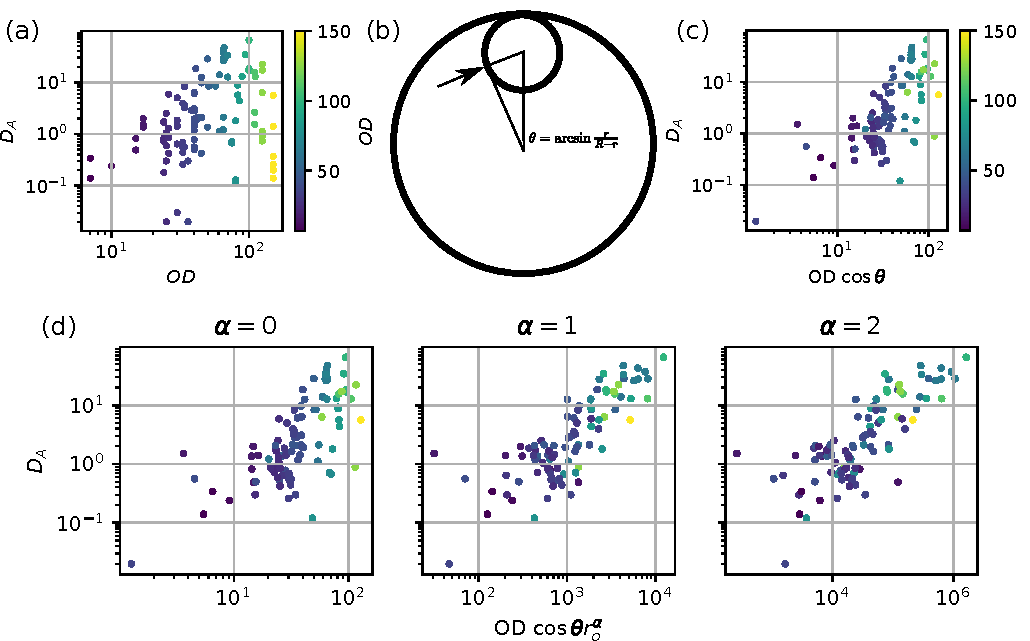
\includegraphics[width=\textwidth]{collision-angle-figure}
  \caption{Saturation time $\tilde\tau$ as a function of geometrical factor $(r_o-r_i)/r_i^2$.}
  \label{fig:collision-angle}
\end{figure*}



% Now we can study the limits cases as:
% For short's times $t \to 0$:s
% \begin{equation}
% 	\label{tcortos}
% 	\left<\Delta x^2\right>\approx v_b^2 t^2.
% \end{equation}
% For $t \to \infty$:
% \begin{equation}
% 	\label{tlargos}
% 	\left<\Delta x^2\right>\approx \frac{v_b^2}{\frac{1}{\tilde{\tau}}(\frac{1}{\tau}+\frac{1}{\tilde{\tau}})}.
% \end{equation}
% We can see that for short times, the MSD has a ballistic behavior, and for long times the MSD saturates.







\appendix

\section{Droplet tracking}

Although the HT method can roughly detect the locations of the inner droplets, the accuracy was not satisfactory when we just use it as it was. 
There are two major issues: 
(i) No subpixel accuracy: all the detections are separated from each other by integer pixels; (ii) Inconsistent detection: whether the algorithm detects the inner edge or the outer edge of a droplet is not consistent, essentially because it only considers the pixel intensity gradient.

\begin{figure}[!t]
  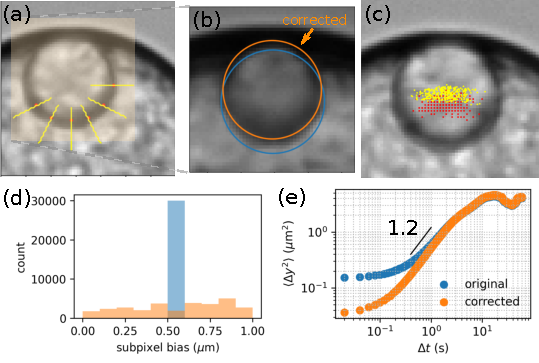
\includegraphics[width=\columnwidth]{hc-correction}
  \caption{
  \textbf{A custom method to improve tracking accuracy of HT method.}
  (a) Illustration of cross-boundary intensity profiles.
  (b) Original detection (blue) and corrected detection (orange).
  (c) Original trajectory (red) and corrected trajectory (yellow).
  (d) Subpixel bias of original trajectory (blue) and improved trajectory (orange).
  (e) MSD of original trajectory (blue) and improved trajectory (orange).
  }
  \label{fig:hc-correction}
\end{figure}

To resolve these issues, we build a custom correction method to refine the results by HT.
In our images of droplets, we notice that all the droplets have dark edges, which may be a result of strong refraction at the edges. 
If we draw a line from droplet center, in the radial direction, to outside the droplet (yellow lines in Fig.~\ref{fig:hc-correction}(a)), the image intensity profile along that line would likely show a valley (a dark peak, indicated as red spots in Fig.~\ref{fig:hc-correction}(a)). 
This valley turns out to be a more unambiguous indicator of the droplet edge position. 
By drawing multiple lines across the droplet boundary and analyzing each pixel intensity profile to get a valley position, we get the coordinates of multiple points on the
droplet edge, from which we can fit a circle.
As shown in Fig.~\ref{fig:hc-correction}(b), the orange circle is a result of the above fitting procedure.
Compare to the original detection of the HT method (blue circle in Fig.~\ref{fig:hc-correction}(b)), both the size and the position are more consistent with the image. 
Figure~\ref{fig:hc-correction}(c) shows the trajectories from both methods (red for original HT, yellow for corrected).
Two improvements are immediately noticed: 
(i) the corrected trajectory is generally higher, closer to the actual center of the droplet;
(ii) the ``lattice'' like pattern in the original trajectory is absent in corrected trajectory, suggesting less subpixel bias.
Indeed, the subpixel statistics is shown in Fig.~\ref{fig:hc-correction}, and we see considerable improvement on the subpixel bias. 
We compared the MSD of both trajectories, as shown in Fig.~\ref{fig:hc-correction}(e).
At short times, the corrected MSD is generally smaller, while at long times, the two MSD are indistinguishable. 
This difference is expected: HT does not detect droplet location accurately. 
At each step, it adds uncertainty to the detected location, making the short time displacement artificially larger.
At long times, however, this artificial displacement becomes less important compared to the actual displacement, so that the two MSD converge.
Interestingly, both MSD exhibit subdiffusive regimes at short times, suggesting that even the corrected trajectory is subject to detection noise.
It is challenging to eliminate detection noise by further correction of the trajectories.
Therefore, we acknowledge the presence of this noise and incorporate it in our model to fit experimental MSD.
The results are satisfactory.  

\section{Image analysis}
\label{img.analisis}
Videos are shot between 30-70 fps, with the majority shot at 50 fps for 10 minutes, therefore, to extract the position of the outer and inner droplet we have to analyze about 30000 images. 
To do that, we made a tracking script in Matlab thats detect both droplets using a Matlab function  called \textit{imfindcircles}. This function finds circles of given radius range and with certain contrast. 
So we can find dark circles or bright circles of given radii, more parameters can be added to the function, such as sensitivity. The steps to perform the detection of the droplets are summarized in the figure (\ref{Deteccion}). The steps to track the droplets  are: The initial image is cropped  to make detection less resource-intensive, the Matlab \textit{Drawcircle} function is used on this image  to compute the diameter and center of the outer and inner  droplet. From the center and radii of the inner droplet we make a template of the inner droplet with a size of  1.2 times the  inner radii. Now we perform some image adjustments to increase the contrast  and  make the detection easier.  Then using the function \texttt{imfindcircles} for the inner droplet and the outer droplet. For the inner droplet we give to the function a parameter of the radios  $r_{i} \pm$\texttt{delta}, where \texttt{delta} is a constant times the radius detected in the image $k-1$.  We are detecting the inner droplet in the template image, in the step $k$ the template image is compared with the image in the step $k-1$ using the crosscorrelation function \texttt{corr2}.   This function gives a value between $[0-1]$, if this value is $1$ then the image is identical to the image  in the step before. We put the condition if this value is less than 0.5 then increase the value of  \texttt{delta} and so on. The function \texttt{imfindcircles} will detect in a ranges of radius, so in two consecutive image this value of radius can change and therefore change the center of the inner droplet in a small quantity. 

\begin{figure}[b!]
  \includegraphics[width=\columnwidth]{proceso_deteccion}	
  \caption[Detection]{
    \textbf{Tracking. -} 
    From left to right: The initial image is cropped.  
    Then draw two circles to calculate the diameters of the drops. 
    An inner droplet template is created with a size of 1.2 times the radii of the inner droplet. 
    Then we detect the outer drop using \textit{imfindcircles} over the cropped image and the same over the template of the inner droplet.   
    }
		\label{Deteccion}
\end{figure}

After detection, on the raw data the data can be smoothed to remove small fluctuations, but the question now arises, how much can we smooth so as not to remove information about the internal droplet motion?.

\section{Smoothdata analysis}
\label{smoothdata}
\textcolor{red}{Need revision, the language is unclear and may have grammar problems.}
We want to study how data smoothing through affects the measured observables. 
The \textit{smoothdata} function is the function included in the Matlab toolbox, which, as shown in the figure \ref{Datos_videos} the unanalyzed position shows large variations that as the window size increases for the smoothdata function decrease. 
%
The smoothdata function returns a moving average of the elements of the position vector determined by one. 
In the data we have used the \text{Gaussian} method which weights the window with a Gaussian weight.
The \textit{smoothn} function provides a discrete, robust, unsupervised and fast smoothing method for arbitrary-dimensional data of arbitrary dimension.

The videos will show the result of the detection of the internal droplet, the difference of the position between two positions $\Delta X = X_{n+1}-X_{n}$, the X and Y position in time where the time axis moves with the data and a cropping of the internal droplet in time where the image axes remain fixed according to the position of the center of the internal droplet in the initial image plus 1.1 times its radius. (see videos frame by frame)
\begin{figure}[b]
	\includegraphics[width=\columnwidth]{Datos_video}
	\caption{Example analysis of a video, x-position and velocity autocorrelation function for different values of smoothdata and for smoothn function without any input and with robust method.}
	\label{Datos_videos}
\end{figure}


\onecolumngrid
\section{MSD computation}
\begin{equation}
	\label{langevin}
	\dot{x}=u(t)-\frac{1}{\tilde{\tau}} x,
\end{equation} 
We can solve this using the Laplace transform, then $x(t)$ is:
\begin{equation}
	x(t)  = x_0 e^{-\frac{1}{\tilde{\tau}} t}+\int_{0}^{t}e^{-\frac{1}{\tilde{\tau}}(t-s)}u(s)\, ds,
\end{equation}
We will assume that the noise autocorrelation is of the form $\left<u(t)u(t')\right>=v_b^2e^{-|t-t'|/\tau}$, where $v_b^2$ is the noise amplitude and $\tau$ is the persistence time. Also, we will assume that the initial position is independent of the noise, $\left<x(0)u(t)\right>=0$. Having this we can compute the mean square displacement (MSD) as:
\begin{equation}
	\left<\Delta x^2\right>=2e^{-\frac{1}{\tilde{\tau}} t} \int_{0}^{t}ds\, e^{-\frac{1}{\tilde{\tau}}(t-s)}\left<x(0)u(t)\right> +\int_{0}^{t}\int_{0}^{t} ds_1 \, ds_2 e^{-\frac{1}{\tilde{\tau}}(t-s_1)}e^{-\frac{1}{\tilde{\tau}}(t-s_2)}u(s_1)u(s_2)
\end{equation}
\begin{equation}
	\left<\Delta x^2\right>=\int_{0}^{t}\int_{0}^{t} ds_1 \, ds_2 e^{-\frac{1}{\tilde{\tau}}(t-s_1)}e^{-\frac{1}{\tilde{\tau}}(t-s_2)}u(s_1)u(s_2)\, ds_1 ds_2
\end{equation}
\begin{equation}
	\left<\Delta x^2\right>=\int_{0}^{t}\int_{0}^{t}ds_1 \, ds_2\, e^{-\frac{1}{\tilde{\tau}}(t-s_1)}e^{-\frac{1}{\tilde{\tau}}(t-s_2)}e^{-|s_1-s_2|/\tau},
\end{equation}
for the integration, we will use:\\
\includegraphics[width=3cm]{Integracion.png}\\
and the integral change as$\int_{0}^{t} ds_1 \int_{0}^{t} ds2= 2 \int_{0}^{t}ds_1 {\int_{0}^{s_1}}  ds_2$, with  $s_1>s_2$ and then $e^{-|s_1-s_2|/\tau}=e^{-(s_1-s_2)/\tau}$.
we have: 

\begin{equation}
	\left<\Delta x^2\right>=\int_{0}^{t}ds_1\int_{0}^{s_1} \, ds_2\, e^{-\frac{1}{\tilde{\tau}}(t-s_1)}e^{-\frac{1}{\tilde{\tau}}(t-s_2)}e^{-(s_1-s_2)\frac{1}{\tau}},
\end{equation}
After the integration, the MSD is:

\begin{equation}
	\label{MSD}
	\left<\Delta x^2\right>=\frac{2v_b^2}{(\frac{1}{\tilde{\tau}}+\frac{1}{\tau})}\left[\frac{1}{2\frac{1}{\tilde{\tau}}}(1-e^{-2\frac{1}{\tilde{\tau}} t})-\frac{1}{\frac{1}{\tilde{\tau}}-\frac{1}{\tau}}(e^{-(\frac{1}{\tilde{\tau}}+\frac{1}{\tau})t}-e^{-2\frac{1}{\tilde{\tau}} t})\right],
\end{equation}
Expanding the equation to study the limits cases.
\begin{equation}
	=\frac{v_b^2}{\frac{1}{\tilde{\tau}}(\frac{1}{\tilde{\tau}}+\frac{1}{\tau})}-\frac{v_b^2e^{-2\frac{1}{\tilde{\tau}} t}}{\frac{1}{\tilde{\tau}}(\frac{1}{\tilde{\tau}}+\frac{1}{\tau})}+\frac{2v_b^2e^{-2\frac{1}{\tilde{\tau}} t}}{(\frac{1}{\tilde{\tau}}-\frac{1}{\tau})(\frac{1}{\tilde{\tau}}+\frac{1}{\tau})}-\frac{2v_b^2e^{-(\frac{1}{\tilde{\tau}}+\frac{1}{\tau}) t}}{(\frac{1}{\tilde{\tau}}-\frac{1}{\tau})(\frac{1}{\tilde{\tau}}+\frac{1}{\tau})}
\end{equation}
Now we can study the limits cases as:
For short's times $t \to 0$:
\begin{equation}
	\label{tcortos}
	\left<\Delta x^2\right>\approx v_b^2 t^2.
\end{equation}
For $t \to \infty$:
\begin{equation}
	\label{tlargos}
	\left<\Delta x^2\right>\approx \frac{v_b^2}{\frac{1}{\tilde{\tau}}(\frac{1}{\tau}+\frac{1}{\tilde{\tau}})}.
\end{equation}
We can see that for short times, the MSD has a ballistic behavior, and for long times the MSD saturates. We will compute the velocity autocorrelation  $C(t,t') = \left< v(t)v(t')\right>$ using the equation \ref{langevin} with an initial condition in the infinity. The solution of the equation with this initial condition is:

\begin{equation}
	\label{solinfinity}
	x(t)=\int_{-\infty}^{t}e^{-\frac{1}{\tilde{\tau}}(t-s)}  u(s)\, ds.
\end{equation}
The velocity autocorrelation function is: 

\begin{equation}
	C(t,t')= \left< v(t)v(t')\right>=\left<(u(t)-\frac{1}{\tilde{\tau}} x(t))(u(t')-\frac{1}{\tilde{\tau}} x(t'))\right>,
\end{equation}

\begin{equation}
	C(t,t') = \left<u(t)u(t')\right>- \frac{1}{\tilde{\tau}} \left<u(t)x(t')\right>- \frac{1}{\tilde{\tau}} \left<x(t)u(t')\right>+\frac{1}{\tilde{\tau}^2}  \left<x(t)x(t')\right>.
\end{equation}

The first term is the noise autocorrelation $\left<u(t)u(t')\right> =v_b^2 e^{-\frac{1}{\tilde{\tau}}|t-t'|}$. To solve the integrals, we will assume that $t>t'$.

The integral $\left<x(t)u(t')\right>$:
\begin{align}
	\left<x(t)u(t')\right> &= v_b^2\int_{-\infty}^{t}ds \  e^{-\frac{1}{\tilde{\tau}}(t-s)}e^{-\frac{1}{\tau}|t'-s|}, \ \ \ t>t'\\
	&=v_b^2\int_{-\infty}^{t'}ds \ e^{-\frac{1}{\tilde{\tau}}(t-s)-\frac{1}{\tau}(t'-s)}+v_b^2\int_{t'}^{t}ds \ e^{-\frac{1}{\tilde{\tau}}(t-s)-\frac{1}{\tau}(s-t')}, \\
	&=\frac{v_b^2e^{-\frac{1}{\tilde{\tau}}(t-t')}}{\frac{1}{\tilde{\tau}}+\frac{1}{\tau}}+\frac{v_b^2e^{-\frac{1}{\tau}(t-t')}-v_b^2e^{-\frac{1}{\tilde{\tau}}(t-t')}}{\frac{1}{\tilde{\tau}}-\frac{1}{\tau}}.
\end{align}
The second term integral is:
\begin{align}
	\left<u(t)x(t')\right> &= \int_{-\infty}^{t'}ds \ e^{-\frac{1}{\tilde{\tau}}(t'-s)}e^{-\frac{1}{\tau}(t-s)},\\
	&=\frac{e^{-\frac{1}{\tau}(t-t')}}{\frac{1}{\tilde{\tau}}+\frac{1}{\tau}}.
\end{align}

And the last integral:

\begin{align}
	\left<x(t)x(t')\right> &= \int_{-\infty}^{t}ds \ \int_{-\infty}^{t'}ds' \ e^{-\frac{1}{\tilde{\tau}}(t-s)}e^{-\frac{1}{\tilde{\tau}}(t'-s')}e^{-\frac{1}{\tau}|s-s'|},  \\
\end{align}

Where we will use the same procedure as before to change the limits of integration. We have first:
\begin{align}
	C_{I} &= \int_{-\infty}^{t'}ds \ \int_{-\infty}^{t'} ds' \ e^{-\frac{1}{\tilde{\tau}}(t-s)}e^{-\frac{1}{\tilde{\tau}}(t'-s')}e^{-\frac{1}{\tau}(s'-s)},\\
	&=\int_{-\infty}^{t'}ds \ \int_{s}^{t'}ds' \ e^{(\frac{1}{\tilde{\tau}}+\frac{1}{\tau})s}e^{(\frac{1}{\tilde{\tau}}-\frac{1}{\tau})s'}e^{-\frac{1}{\tilde{\tau}} t}e^{-\frac{1}{\tilde{\tau}} t'},\\
	&=\frac{1}{\frac{1}{\tilde{\tau}} - \frac{1}{\tau}}\int_{-\infty}^{t'} ds \ \left[e^{(\frac{1}{\tilde{\tau}}-\frac{1}{\tau})t'}e^{(\frac{1}{\tilde{\tau}}+\frac{1}{\tau})s}-e^{2\frac{1}{\tilde{\tau}} s}\right],\\
	&=\frac{e^{-\frac{1}{\tilde{\tau}}(t-t')}}{\frac{1}{\tilde{\tau}}-\frac{1}{\tau}}\left(\frac{1}{\frac{1}{\tilde{\tau}}+\frac{1}{\tau}}-\frac{1}{2\frac{1}{\tilde{\tau}}}\right).
\end{align}
The next part of the integral is:
\begin{align}
	C_{II} &= \int_{-\infty}^{t'}ds' \ \int_{s'}^{t} ds \ e^{-\frac{1}{\tilde{\tau}}(t-s)}e^{-\frac{1}{\tilde{\tau}}(t'-s')}e^{-\frac{1}{\tau}(s-s')},\\
	&=e^{-\frac{1}{\tilde{\tau}} t-\frac{1}{\tilde{\tau}} t'}\int_{-\infty}^{t'}ds'\ \int_{s'}^{t}ds\ e^{(\frac{1}{\tilde{\tau}}-\frac{1}{\tau})s}e^{(\frac{1}{\tilde{\tau}} +\frac{1}{\tau})s'},\\
	&=\frac{e^{-\frac{1}{\tilde{\tau}} t - \frac{1}{\tilde{\tau}} t'}}{\frac{1}{\tilde{\tau}}-\frac{1}{\tau}}\int_{-\infty}^{t'}ds'\ \left[e^{(\frac{1}{\tilde{\tau}}-\frac{1}{\tau})t}e^{(\frac{1}{\tilde{\tau}}+\frac{1}{\tau})s'}-e^{\frac{2}{\tilde{\tau}} s'}\right],\\
	&=\frac{1}{(\frac{1}{\tilde{\tau}}-\frac{1}{\tau})(\frac{1}{\tilde{\tau}}+\frac{1}{\tau})}e^{-\frac{1}{\tau}(t-t')}-\frac{1}{\frac{2}{\tilde{\tau}}(\frac{1}{\tilde{\tau}}-\frac{1}{\tau})}e^{-\frac{1}{\tilde{\tau}}(t-t')}.
\end{align}
Bringing together all the terms, the velocity autocorrelation function is:

\begin{equation}
	C(t,t')= \frac{v_b^2}{(\frac{1}{\tilde{\tau}}+\frac{1}{\tau})(\frac{1}{\tilde{\tau}}-\frac{1}{\tau})}\left[\left(\frac{1}{\tilde{\tau}^2} + \frac{\frac{1}{\tilde{\tau}}}{\tau} -\frac{1}{\tau^2}\right)e^{-\frac{1}{\tilde{\tau}}(t-t')}-\frac{1}{\tilde{\tau}^2} e^{-\frac{1}{\tau}(t-t')}\right], \ \ t > t'
\end{equation}
For $t=t'$

\begin{equation}
	C(t,t)= \langle v^2 \rangle = \frac{v_b^2}{\frac{1}{\tilde{\tau}} \tau+1}=\frac{v_b^2\tilde{\tau}}{\tau+\tilde{\tau}}, \ \ 
\end{equation}









\bibliography{ref}



\end{document}
%
% ****** End of file apssamp.tex ******